\documentclass{ximera}

%\usepackage{todonotes}

\newcommand{\todo}{}

\usepackage{esint} % for \oiint
\ifxake%%https://math.meta.stackexchange.com/questions/9973/how-do-you-render-a-closed-surface-double-integral
\renewcommand{\oiint}{{\large\bigcirc}\kern-1.56em\iint}
\fi


\graphicspath{
  {./}
  {ximeraTutorial/}
  {basicPhilosophy/}
  {functionsOfSeveralVariables/}
  {normalVectors/}
  {lagrangeMultipliers/}
  {vectorFields/}
  {greensTheorem/}
  {shapeOfThingsToCome/}
  {dotProducts/}
  {partialDerivativesAndTheGradientVector/}
  {../productAndQuotientRules/exercises/}
  {../normalVectors/exercisesParametricPlots/}
  {../continuityOfFunctionsOfSeveralVariables/exercises/}
  {../partialDerivativesAndTheGradientVector/exercises/}
  {../directionalDerivativeAndChainRule/exercises/}
  {../commonCoordinates/exercisesCylindricalCoordinates/}
  {../commonCoordinates/exercisesSphericalCoordinates/}
  {../greensTheorem/exercisesCurlAndLineIntegrals/}
  {../greensTheorem/exercisesDivergenceAndLineIntegrals/}
  {../shapeOfThingsToCome/exercisesDivergenceTheorem/}
  {../greensTheorem/}
  {../shapeOfThingsToCome/}
  {../separableDifferentialEquations/exercises/}
  {vectorFields/}
}

\newcommand{\mooculus}{\textsf{\textbf{MOOC}\textnormal{\textsf{ULUS}}}}

\usepackage{tkz-euclide}
\usepackage{tikz}
\usepackage{tikz-cd}
\usetikzlibrary{arrows}
\tikzset{>=stealth,commutative diagrams/.cd,
  arrow style=tikz,diagrams={>=stealth}} %% cool arrow head
\tikzset{shorten <>/.style={ shorten >=#1, shorten <=#1 } } %% allows shorter vectors

\usetikzlibrary{backgrounds} %% for boxes around graphs
\usetikzlibrary{shapes,positioning}  %% Clouds and stars
\usetikzlibrary{matrix} %% for matrix
\usepgfplotslibrary{polar} %% for polar plots
\usepgfplotslibrary{fillbetween} %% to shade area between curves in TikZ
%\usetkzobj{all}
\usepackage[makeroom]{cancel} %% for strike outs
%\usepackage{mathtools} %% for pretty underbrace % Breaks Ximera
%\usepackage{multicol}
\usepackage{pgffor} %% required for integral for loops



%% http://tex.stackexchange.com/questions/66490/drawing-a-tikz-arc-specifying-the-center
%% Draws beach ball
\tikzset{pics/carc/.style args={#1:#2:#3}{code={\draw[pic actions] (#1:#3) arc(#1:#2:#3);}}}



\usepackage{array}
\setlength{\extrarowheight}{+.1cm}
\newdimen\digitwidth
\settowidth\digitwidth{9}
\def\divrule#1#2{
\noalign{\moveright#1\digitwidth
\vbox{\hrule width#2\digitwidth}}}




% \newcommand{\RR}{\mathbb R}
% \newcommand{\R}{\mathbb R}
% \newcommand{\N}{\mathbb N}
% \newcommand{\Z}{\mathbb Z}

\newcommand{\sagemath}{\textsf{SageMath}}


%\renewcommand{\d}{\,d\!}
%\renewcommand{\d}{\mathop{}\!d}
%\newcommand{\dd}[2][]{\frac{\d #1}{\d #2}}
%\newcommand{\pp}[2][]{\frac{\partial #1}{\partial #2}}
% \renewcommand{\l}{\ell}
%\newcommand{\ddx}{\frac{d}{\d x}}

% \newcommand{\zeroOverZero}{\ensuremath{\boldsymbol{\tfrac{0}{0}}}}
%\newcommand{\inftyOverInfty}{\ensuremath{\boldsymbol{\tfrac{\infty}{\infty}}}}
%\newcommand{\zeroOverInfty}{\ensuremath{\boldsymbol{\tfrac{0}{\infty}}}}
%\newcommand{\zeroTimesInfty}{\ensuremath{\small\boldsymbol{0\cdot \infty}}}
%\newcommand{\inftyMinusInfty}{\ensuremath{\small\boldsymbol{\infty - \infty}}}
%\newcommand{\oneToInfty}{\ensuremath{\boldsymbol{1^\infty}}}
%\newcommand{\zeroToZero}{\ensuremath{\boldsymbol{0^0}}}
%\newcommand{\inftyToZero}{\ensuremath{\boldsymbol{\infty^0}}}



% \newcommand{\numOverZero}{\ensuremath{\boldsymbol{\tfrac{\#}{0}}}}
% \newcommand{\dfn}{\textbf}
% \newcommand{\unit}{\,\mathrm}
% \newcommand{\unit}{\mathop{}\!\mathrm}
% \newcommand{\eval}[1]{\bigg[ #1 \bigg]}
% \newcommand{\seq}[1]{\left( #1 \right)}
% \renewcommand{\epsilon}{\varepsilon}
% \renewcommand{\phi}{\varphi}


% \renewcommand{\iff}{\Leftrightarrow}

% \DeclareMathOperator{\arccot}{arccot}
% \DeclareMathOperator{\arcsec}{arcsec}
% \DeclareMathOperator{\arccsc}{arccsc}
% \DeclareMathOperator{\si}{Si}
% \DeclareMathOperator{\scal}{scal}
% \DeclareMathOperator{\sign}{sign}


%% \newcommand{\tightoverset}[2]{% for arrow vec
%%   \mathop{#2}\limits^{\vbox to -.5ex{\kern-0.75ex\hbox{$#1$}\vss}}}
% \newcommand{\arrowvec}[1]{{\overset{\rightharpoonup}{#1}}}
% \renewcommand{\vec}[1]{\arrowvec{\mathbf{#1}}}
% \renewcommand{\vec}[1]{{\overset{\boldsymbol{\rightharpoonup}}{\mathbf{#1}}}}

% \newcommand{\point}[1]{\left(#1\right)} %this allows \vector{ to be changed to \vector{ with a quick find and replace
% \newcommand{\pt}[1]{\mathbf{#1}} %this allows \vec{ to be changed to \vec{ with a quick find and replace
% \newcommand{\Lim}[2]{\lim_{\point{#1} \to \point{#2}}} %Bart, I changed this to point since I want to use it.  It runs through both of the exercise and exerciseE files in limits section, which is why it was in each document to start with.

% \DeclareMathOperator{\proj}{\mathbf{proj}}
% \newcommand{\veci}{{\boldsymbol{\hat{\imath}}}}
% \newcommand{\vecj}{{\boldsymbol{\hat{\jmath}}}}
% \newcommand{\veck}{{\boldsymbol{\hat{k}}}}
% \newcommand{\vecl}{\vec{\boldsymbol{\l}}}
% \newcommand{\uvec}[1]{\mathbf{\hat{#1}}}
% \newcommand{\utan}{\mathbf{\hat{t}}}
% \newcommand{\unormal}{\mathbf{\hat{n}}}
% \newcommand{\ubinormal}{\mathbf{\hat{b}}}

% \newcommand{\dotp}{\bullet}
% \newcommand{\cross}{\boldsymbol\times}
% \newcommand{\grad}{\boldsymbol\nabla}
% \newcommand{\divergence}{\grad\dotp}
% \newcommand{\curl}{\grad\cross}
%\DeclareMathOperator{\divergence}{divergence}
%\DeclareMathOperator{\curl}[1]{\grad\cross #1}
% \newcommand{\lto}{\mathop{\longrightarrow\,}\limits}

% \renewcommand{\bar}{\overline}

\colorlet{textColor}{black}
\colorlet{background}{white}
\colorlet{penColor}{blue!50!black} % Color of a curve in a plot
\colorlet{penColor2}{red!50!black}% Color of a curve in a plot
\colorlet{penColor3}{red!50!blue} % Color of a curve in a plot
\colorlet{penColor4}{green!50!black} % Color of a curve in a plot
\colorlet{penColor5}{orange!80!black} % Color of a curve in a plot
\colorlet{penColor6}{yellow!70!black} % Color of a curve in a plot
\colorlet{fill1}{penColor!20} % Color of fill in a plot
\colorlet{fill2}{penColor2!20} % Color of fill in a plot
\colorlet{fillp}{fill1} % Color of positive area
\colorlet{filln}{penColor2!20} % Color of negative area
\colorlet{fill3}{penColor3!20} % Fill
\colorlet{fill4}{penColor4!20} % Fill
\colorlet{fill5}{penColor5!20} % Fill
\colorlet{gridColor}{gray!50} % Color of grid in a plot

\newcommand{\surfaceColor}{violet}
\newcommand{\surfaceColorTwo}{redyellow}
\newcommand{\sliceColor}{greenyellow}




\pgfmathdeclarefunction{gauss}{2}{% gives gaussian
  \pgfmathparse{1/(#2*sqrt(2*pi))*exp(-((x-#1)^2)/(2*#2^2))}%
}


%%%%%%%%%%%%%
%% Vectors
%%%%%%%%%%%%%

%% Simple horiz vectors
\renewcommand{\vector}[1]{\left\langle #1\right\rangle}


%% %% Complex Horiz Vectors with angle brackets
%% \makeatletter
%% \renewcommand{\vector}[2][ , ]{\left\langle%
%%   \def\nextitem{\def\nextitem{#1}}%
%%   \@for \el:=#2\do{\nextitem\el}\right\rangle%
%% }
%% \makeatother

%% %% Vertical Vectors
%% \def\vector#1{\begin{bmatrix}\vecListA#1,,\end{bmatrix}}
%% \def\vecListA#1,{\if,#1,\else #1\cr \expandafter \vecListA \fi}

%%%%%%%%%%%%%
%% End of vectors
%%%%%%%%%%%%%

%\newcommand{\fullwidth}{}
%\newcommand{\normalwidth}{}



%% makes a snazzy t-chart for evaluating functions
%\newenvironment{tchart}{\rowcolors{2}{}{background!90!textColor}\array}{\endarray}

%%This is to help with formatting on future title pages.
\newenvironment{sectionOutcomes}{}{}



%% Flowchart stuff
%\tikzstyle{startstop} = [rectangle, rounded corners, minimum width=3cm, minimum height=1cm,text centered, draw=black]
%\tikzstyle{question} = [rectangle, minimum width=3cm, minimum height=1cm, text centered, draw=black]
%\tikzstyle{decision} = [trapezium, trapezium left angle=70, trapezium right angle=110, minimum width=3cm, minimum height=1cm, text centered, draw=black]
%\tikzstyle{question} = [rectangle, rounded corners, minimum width=3cm, minimum height=1cm,text centered, draw=black]
%\tikzstyle{process} = [rectangle, minimum width=3cm, minimum height=1cm, text centered, draw=black]
%\tikzstyle{decision} = [trapezium, trapezium left angle=70, trapezium right angle=110, minimum width=3cm, minimum height=1cm, text centered, draw=black]


\title{Theory}

\begin{document}

\begin{abstract}
the exponential story
\end{abstract}
\maketitle





We have two levels of exponential formulas: the basic template and then the general template, which includes shifts and stretches.  All of these are based on our original idea of \textbf{\textcolor{purple!85!blue}{constant percentage growth}}.


Constant percentage growth means that the value  of our function grows by an equal percentage over equal size intervals in the domain.



For example, let $f$ be a function that grows by $30\%$ over every domain interval of length $1$. \\


\begin{itemize}
\item If $f(0) = 1$, then $f(1) = 1.3 \cdot 1 = 1.3$
\item If $f(5) = 21$, then $f(6) = 1.3 \cdot 21 = 27.3$
\item If $f(\pi) = \sqrt{3}$, then $f(\pi + 1) = 1.3 \cdot \sqrt{3} = 1.3 \sqrt{3}$
\end{itemize}

Every time the domain interval changes by $1$, then the function value is multiplied by $1.3$ (an increase of $30\%$).






For example, let $g$ be a function that grows by $10\%$ over every domain interval of length $3$. \\


\begin{itemize}
\item If $g(0) = 5$, then $g(3) = 1.1 \cdot 5  = 5.5$
\item If $g(5) = 16$, then $g(8) = 1.1 \cdot 16  = 17.6$
\item If $g(\sqrt{3}) = 7$, then $g(\sqrt{3} + 3) = 1.1 \cdot 7 = 7.7$
\end{itemize}

Every time the domain interval changes by $3$, then the function value is multiplied by $1.1$ (an increase (change) of $10\%$).







There are many basic exponential functions that possess this characteristic. They all can be written in the form \textbf{\textcolor{blue!55!black}{$f(x) = a \cdot r^x$}}. 

We call \textbf{\textcolor{purple!85!blue}{$a=f(0)$}} the \textbf{\textcolor{purple!85!blue}{initial value}}. \\

We call \textbf{\textcolor{purple!85!blue}{$r$}} the \textbf{\textcolor{purple!85!blue}{base}}.  It tells us how fast the function grows.







\begin{image}
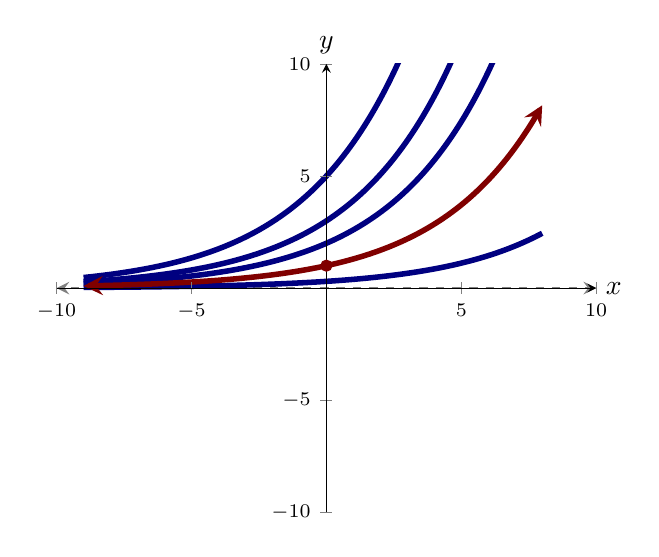
\begin{tikzpicture}
   \begin{axis}[name = leftgraph, 
            domain=-10:10, ymax=10, xmax=10, ymin=-10, xmin=-10,
            axis lines =center, xlabel=$x$, ylabel={$y$},
            ticklabel style={font=\scriptsize},
            every axis y label/.style={at=(current axis.above origin),anchor=south},
            every axis x label/.style={at=(current axis.right of origin),anchor=west},
            axis on top
          ]
          
          \addplot [line width=1, gray, dashed,samples=200,domain=(-10:10),<->] {0};


          \addplot [line width=2, penColor, smooth,samples=100,domain=(-9:8)] {2 * (1.3^x)};
          \addplot [line width=2, penColor, smooth,samples=100,domain=(-9:8)] {3 * (1.3^x)};
          \addplot [line width=2, penColor, smooth,samples=100,domain=(-9:8)] {5 * (1.3^x)};
          \addplot [line width=2, penColor, smooth,samples=100,domain=(-9:8)] {0.3 * (1.3^x)};

          \addplot [line width=2, penColor2, smooth,samples=100,domain=(-9:8), <->] {1.3^x};
          \addplot [color=penColor2,only marks,mark=*] coordinates{(0,1)};

  \end{axis}
\end{tikzpicture}
\end{image}



Functions that possess this constant percentage growth proprty are called exponential formula.

We can think of exponential functions as shifts and stretches of a basic exponential funciton. \\




\subsection*{The Basic Exponential Formula}


The template for the formula of the basic exponential function looks like




\[  a \cdot r^x   \, \text{ with } \,  a, r \in \mathbb{R} \, | \,  a \ne 0, \, r > 0   \]


The \textbf{\textcolor{purple!85!blue}{leading coefficient}}, $a$, controls vertical stretching or compression. The sign of $a$ dictates the sign of our function values, which is illustrated graphically as a vertical reflection. The \textbf{\textcolor{purple!85!blue}{base}}, $r$, dictates a growing or decaying function - the constant prcentage change could be an increase or decrease.




We have four combinations of our coefficient and base parameters.

\begin{itemize}
\item $a>0$ and $r>1$
\item $a>0$ and $r<1$
\item $a<0$ and $r>1$
\item $a<0$ and $r<1$
\end{itemize}


Graphs of the basic exponential functions have the horizontal axis as a horizontal asymptote in one direction or the other.

\begin{explanation}


When $r$ \wordChoice{\choice{$<$} \choice[correct]{$>$}} $1$ we have a growing function. It could be growing positively or negatively, depending on the sign of $a$.

\[  \lim_{x \to -\infty} a \, r^x = 0 \, \text{ and } \, \lim_{x \to \infty} a \, r^x = \pm\infty \]


Since $r^x$ is always positive, it is the sign of $a$ that dictates if the unbounded growth is positive or negative.




\begin{image}
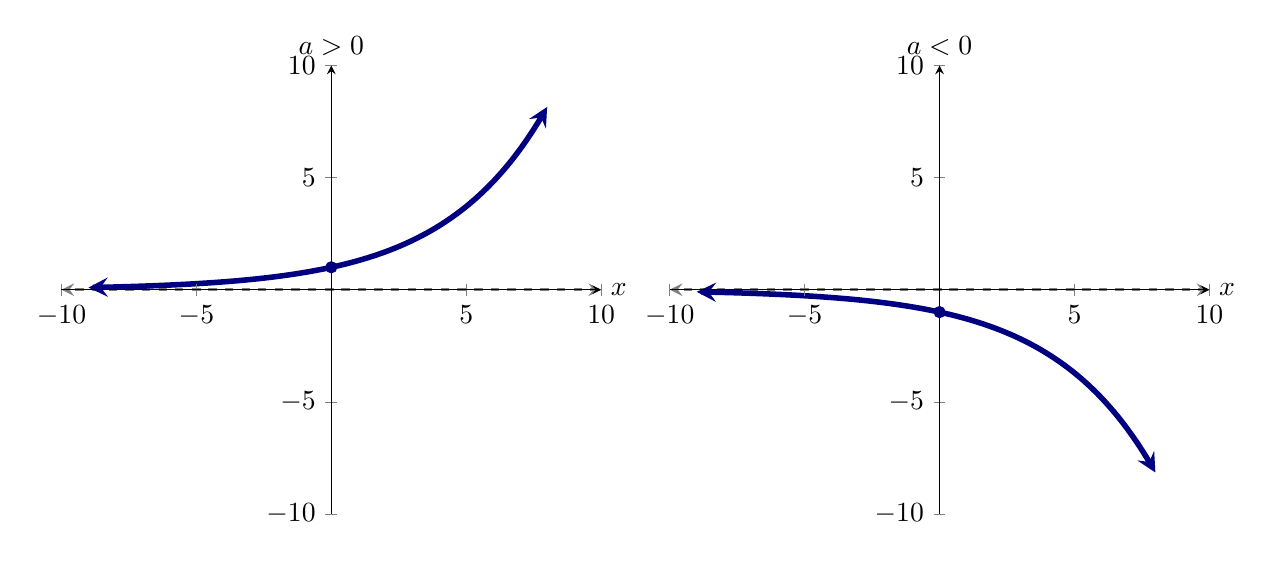
\begin{tikzpicture}
   \begin{axis}[name = leftgraph, 
            domain=-10:10, ymax=10, xmax=10, ymin=-10, xmin=-10,
            axis lines =center, xlabel=$x$, ylabel={$a>0$},
            every axis y label/.style={at=(current axis.above origin),anchor=south},
            every axis x label/.style={at=(current axis.right of origin),anchor=west},
            axis on top
          ]
          
          \addplot [line width=1, gray, dashed,samples=200,domain=(-10:10),<->] {0};

          \addplot [line width=2, penColor, smooth,samples=100,domain=(-9:8), <->] {1.3^x};
          \addplot [color=penColor,only marks,mark=*] coordinates{(0,1)};

           

  \end{axis}
  \begin{axis}[at={(leftgraph.outer east)},anchor=outer west, 
            domain=-10:10, ymax=10, xmax=10, ymin=-10, xmin=-10,
            axis lines =center, xlabel=$x$, ylabel={$a<0$},
            every axis y label/.style={at=(current axis.above origin),anchor=south},
            every axis x label/.style={at=(current axis.right of origin),anchor=west},
            axis on top
          ]
          
          \addplot [line width=1, gray, dashed,samples=200,domain=(-10:10),<->] {0};

          \addplot [line width=2, penColor, smooth,samples=100,domain=(-9:8),<->] {-(1.3^x)};
          \addplot [color=penColor,only marks,mark=*] coordinates{(0,-1)};

           

  \end{axis}
\end{tikzpicture}
\end{image}


Graphs of basic exponential functions have one strategic point, which occurs when the exponent equals zero. For the basic exponential function, this point is $\left( \answer{0}, a \right)$.


Exponential functions have unbounded growth in the direction that makes the exponent large and \wordChoice{\choice[correct]{positive} \choice{negative}}.


Exponential functions approach $0$ in the direction that makes the exponent large and \wordChoice{\choice{positive} \choice[correct]{negative}}.




\end{explanation}





\begin{explanation}



When $r$ \wordChoice{\choice[correct]{$<$} \choice{$>$}} $1$, we have a decaying function. The horizontal axis is still a horizontal asymptote, just in the direction where $x$ is large and positive. The function now decays. It could decay positively or negatively, depending on the sign of $a$.


\[ \lim_{x \to -\infty} a \, r^x = \pm\infty \, \text{ and } \, \lim_{x \to \infty} a \, r^x = 0 \]


 
The sign of $a$ dictates if the function decays through positive or negative values, because $r^x > 0$.



\begin{image}
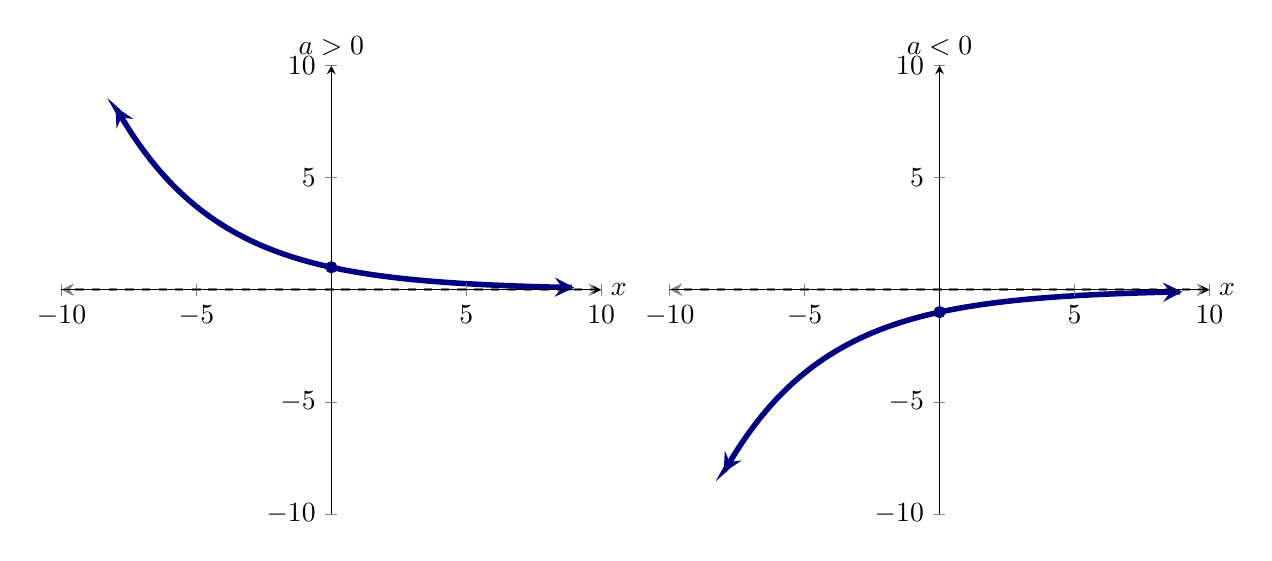
\begin{tikzpicture}
   \begin{axis}[name = leftgraph, 
            domain=-10:10, ymax=10, xmax=10, ymin=-10, xmin=-10,
            axis lines =center, xlabel=$x$, ylabel={$a>0$},
            every axis y label/.style={at=(current axis.above origin),anchor=south},
            every axis x label/.style={at=(current axis.right of origin),anchor=west},
            axis on top
          ]
          
          \addplot [line width=1, gray, dashed,samples=200,domain=(-10:10),<->] {0};

          \addplot [line width=2, penColor, smooth,samples=200,domain=(-8:9), <->] {1.3^(-x)};
          \addplot [color=penColor,only marks,mark=*] coordinates{(0,1)};
           

  \end{axis}
  \begin{axis}[at={(leftgraph.outer east)},anchor=outer west, 
            domain=-10:10, ymax=10, xmax=10, ymin=-10, xmin=-10,
            axis lines =center, xlabel=$x$, ylabel={$a<0$},
            every axis y label/.style={at=(current axis.above origin),anchor=south},
            every axis x label/.style={at=(current axis.right of origin),anchor=west},
            axis on top
          ]
          
          \addplot [line width=1, gray, dashed,samples=200,domain=(-10:10),<->] {0};

          \addplot [line width=2, penColor, smooth,samples=200,domain=(-8:9),<->] {-(1.3^(-x)};
          \addplot [color=penColor,only marks,mark=*] coordinates{(0,-1)};
           

  \end{axis}
\end{tikzpicture}
\end{image}



Graphs of basic exponential functions have one strategic point, which occurs when the exponent equals zero. For the basic exponential function, this point is $(0, a)$, which is below the horizontal asymptote, when $a < 0$.




Exponential functions have unbounded growth in the direction that makes the exponent large and \wordChoice{\choice[correct]{positive} \choice{negative}}.


Exponential functions approach $0$ in the direction that makes the exponent large and \wordChoice{\choice{positive} \choice[correct]{negative}}.


\end{explanation}






All four basic exponential functions share a common structure.


\begin{itemize}
\item Each is always positive or always negative. This depends on the sign of $a$.
\item Each approaches $0$ in one direction - the direction that makes the exponent large and negative.
\item In the other direction, they grow unbounded. 
\end{itemize}





All four basic exponential graphs share a common structure.


\begin{itemize}
\item Each is always above or below the horizontal axis. This depends on the sign of $a$.
\item Each has the horizontal axis as an asymptote in one direction.
\item In the other direction, they grow unbounded. 
\end{itemize}




These are the important aspects or characteristics that we watch when moving onto shifting and stretching the graphs of exponential functions.












\begin{summary} \textbf{\textcolor{blue!75!black}{Exponential Behavior}}


Basic exponential functions, $a \cdot r^x$, are either increasing functions or decreasing functions.


$\blacktriangleright$  \textbf{\textcolor{purple!85!blue}{Base Greater than $1$: $r > 1$}} 


\begin{itemize}
\item greater positive exponents mean multiplying by the base more, which results in larger values.  
\item greater negative exponents mean multiplying by the reciprocal of the base more, which results in smaller values.  
\end{itemize}


The coefficient in front, $a$, tells us if this larger/smaller value is positive or negative.


\begin{itemize}
\item $a > 0$ and $r > 1$ : \wordChoice{\choice[correct]{increasing} \choice{decreasing}}  (positive) function
\item $a < 0$ and $r > 1$ : \wordChoice{\choice{increasing} \choice[correct]{decreasing}}  (negative) function  
\end{itemize}






$\blacktriangleright$  \textbf{\textcolor{purple!85!blue}{Base Less than $1$: $0 < r < 1$}}  


\begin{itemize} 
\item greater positive exponents mean multiplying by the base more, which results in smaller values.  
\item greater negative exponents mean multiplying by the reciprocal of the base more, which results in larger values.  
\end{itemize}


The coefficient in front, $a$, tells us if this larger/smaller value is positive or negative.


\begin{itemize}
\item $a > 0$ and $r < 1$ : \wordChoice{\choice{increasing} \choice[correct]{decreasing}}  (positive) function
\item $a < 0$ and $r < 1$ : \wordChoice{\choice[correct]{increasing} \choice{decreasing}}  (negative) function  
\end{itemize}



\end{summary}




As we see, basic exponential functions can be

\begin{itemize}
\item positive and increasing ($a>0$ and $r>1$)
\item positive and decreasing ($a>0$ and $r<1$)
\item negative and increasing ($a<0$ and $r<1$)
\item negative and decreasing ($a<0$ and $r>1$)
\end{itemize}













\subsection*{Analysis}






\begin{example}  



Analyze   $f(x) = \frac{1}{3} \cdot \, 2^{x+5}$ \\

Categorize: $f$ is an exponential function, because it matches our template for exponential functions, $a \, r^x$.





\begin{idea}

We'll begin by thinking about the graph to help guide our analysis. \\






The ``inside'' (the argument) of the formula for $f(x)$, representing the domain, is $x+5$.  This equals $0$, when $x=-5$.  The exponent is positive for $x>-5$, and because the base is $2 > 1$, this is the direction (right) of unbounded growth.  Therefore, the other direction (left) is where the horizontal asymptote is in effect.  Since the leading coefficient is $\frac{1}{3} > 0$, the unbounded growth is positive.

At $x=-5$, we have our one anchor point for the graph.  The point is $\left(-5, \frac{1}{3} \right)$, which is $\frac{1}{3}$ above the horizontal axis.


Graph of $y = f(x)$.

\begin{image}
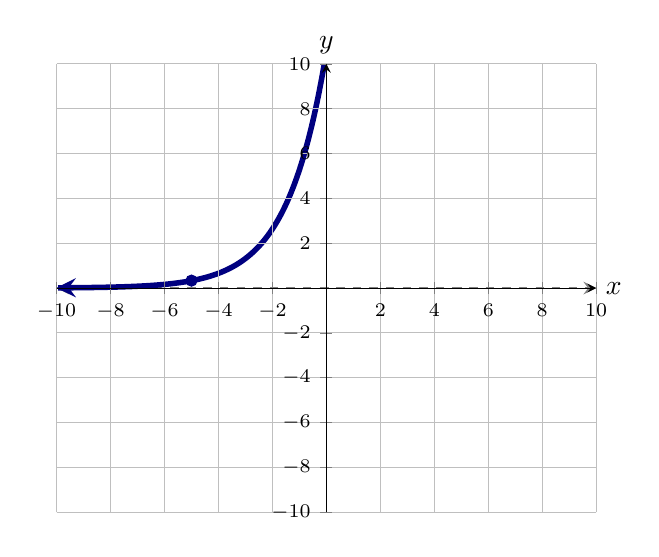
\begin{tikzpicture}
  \begin{axis}[
            domain=-10:10, ymax=10, xmax=10, ymin=-10, xmin=-10,
            axis lines =center, xlabel=$x$, ylabel=$y$, grid = major,
            ytick={-10,-8,-6,-4,-2,2,4,6,8,10},
          	xtick={-10,-8,-6,-4,-2,2,4,6,8,10},
          	ticklabel style={font=\scriptsize},
            every axis y label/.style={at=(current axis.above origin),anchor=south},
            every axis x label/.style={at=(current axis.right of origin),anchor=west},
            axis on top
          ]
          
          \addplot [line width=1, gray, dashed,samples=200,domain=(-10:10),<->] {0};

      	  \addplot [line width=2, penColor, smooth,samples=200,domain=(-10:0.6),<->] {0.33 * 2^(x+5)};

      	  \addplot[color=penColor,fill=penColor,only marks,mark=*] coordinates{(-5,0.333)};

          


 

  \end{axis}
\end{tikzpicture}
\end{image}



\end{idea}


Now, for our (algebraic) function analysis.







\textbf{Domain:} 

The domain of every exponential function is $(-\infty, \infty)$. \\



\textbf{Zeros:}  

Exponential functions do not have zeros. \\


\textbf{Continuity:}  Exponential functions are continuous.  \\



\textbf{End-Behavior:} 

The base of $f$ is $2 > 1$. $2^{positive}$ will get big. $2^{negative}$ will get small. \\ 

The linear exponent of $f$ is $x+5$ has a positive leading coefficient. \\

The negative direction is the direction that makes the exponent large and negative.  That makes this the direction that the function value levels off to $0$. \\


\[
\lim\limits_{x \to -\infty} f(x) = 0
\]




The other direction is where the exponential function is uunbounded.  Since the leading coefficient of $f$ is positive, $f$ is unbounded positively. \\



\[
\lim\limits_{x \to \infty} f(x) = \infty
\]









\textbf{Behavior:} 

The base of $f$ is $2$, which is greter than $1$. The leading coefficient of $f$ is $\frac{1}{3}$, which is positive. The leading coefficient of the linear exponent is $1$, which is also positive.  These make $f$ is a positive increasing exponential function.



\textbf{Global Extrema:}  Exponential functions do not have global maximums or minimums. \\


\textbf{Local Extrema:}  Exponentials functions do not have local maximums or minimums. \\



\textbf{Range:} The end-behavior tells us that the range is $(0, \infty)$.





\end{example}

















$\blacktriangleright$ \textbf{\textcolor{blue!55!black}{Shifting or Not}} \\



Basic exponential functions can swallow up horizontal shifting into the leading coefficient.



If we add/subtract $b$ in the exponent, for a horizontal stretch, then we have

\[
a \cdot r^{x + b} = a \cdot r^x \cdot r^b = a \cdot r^b \cdot r^x = (a \cdot r^b) \cdot r^x
\]

We obtain a new leading coefficient. \\

It just depends on how you like to see exponential functions. \\

















$\blacktriangleright$ \textbf{\textcolor{blue!55!black}{Stretching or Not}} \\



Basic exponential functions swallow up stretching and compressing into the leading coefficient and base.


\begin{itemize}
\item If we multiply on the outside, by $b$, for a vertical stretch, then we have

\[
b \cdot (a \cdot r^x) = (a \cdot b) \cdot r^x
\]

We obtain a new leading coefficient. \\






\item If we multiply on the inside, by $b$, for a horizontal stretch, then our exponential rules give us

\[
a \cdot r^{b \cdot x} = a \cdot (r^b)^x = a \cdot R^x
\]

We obtain a new base, which tells us about the growth of the function.


\end{itemize}


It just depends on how you like to see exponential functions. \\



You should pick a basic basic exponential function to which you will compare other exponential functions.

It is common for students to first select $2^x$. It turns out that $e^x$ will become the focus of our attention in mathematics.  So, it becomes common to select $e^x$ is the basic basic exponential function to memorize. \\


From this choice, there are four immediate configurations from our template, $a \, r^x$.\\




\begin{itemize}
\item  $e^x$ ($a>0$ and $r>1$) positive and increasing
\item  $e^{-x}$ ($a>0$ and $r<1$) positive and decreasing
\item  $-e^x$ ($a<0$ and $r<1$) negative and increasing
\item  $-e^{-x}$ ($a<0$ and $r>1$) negative and decreasing
\end{itemize}


\textbf{Note:}  $e^{-x} = \left( e^{-1} \right)^x = \left( \frac{1}{e} \right)^x$, which is a base less than $1$.


\textbf{Note:}  We also have the option of viewing exponential functions in a more general form, $a \, r^{B \, x + C}$.  With this viewpoint, we would phrase the configurations above as



$r > 1$, the base is greater than $1$, so examine leading coefficients.
\begin{itemize}
\item  $e^x$ ($a>0$ and $B>0$) positive and increasing
\item  $e^{-x}$ ($a>0$ and $B<0$) positive and decreasing
\item  $-e^x$ ($a<0$ and $B>0$) negative and increasing
\item  $-e^{-x}$ ($a<0$ and $B<0$) negative and decreasing
\end{itemize}





It just depends on how you like to see exponential functions. \\













We can use any algebra any time any where that we feel helps us.











\begin{example} 



$f(x) = \frac{1}{3} \, 2^{x+5}$ is the function in the last example.  We could take advantage of exponential algebra to simplify the formula.   \\

\[ 
f(x) = \frac{1}{3} \, 2^{x+5} = \frac{1}{3} \, 2^x \cdot 2^5 = \frac{32}{3} \, 2^x 
\]


The new base is still $2$ and the new leading coefficient is $\frac{32}{3}$ and there is no shifting.  Same function.  Different formula.





From this viewpoint, we change our strategic point to $\left( 0, \frac{32}{3} \right)$.




\begin{image}
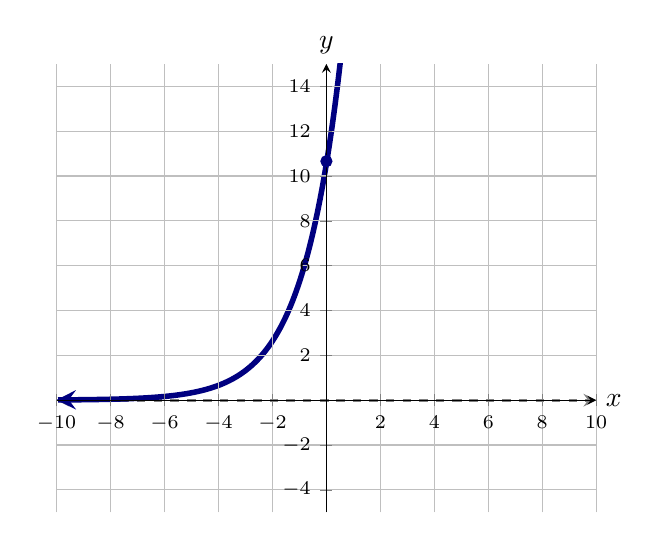
\begin{tikzpicture}
  \begin{axis}[
            domain=-10:10, ymax=15, xmax=10, ymin=-5, xmin=-10,
            axis lines =center, xlabel=$x$, ylabel=$y$, grid = major,
            ytick={-4,-2,2,4,6,8,10,12,14},
            xtick={-10,-8,-6,-4,-2,2,4,6,8,10},
            ticklabel style={font=\scriptsize},
            every axis y label/.style={at=(current axis.above origin),anchor=south},
            every axis x label/.style={at=(current axis.right of origin),anchor=west},
            axis on top
          ]
          
          \addplot [line width=1, gray, dashed,samples=200,domain=(-10:10),<->] {0};

          \addplot [line width=2, penColor, smooth,samples=200,domain=(-10:0.6),<->] {0.33 * 2^(x+5)};

          \addplot[color=penColor,fill=penColor,only marks,mark=*] coordinates{(0,10.66)};

          


 

  \end{axis}
\end{tikzpicture}
\end{image}




Same function.  Different perspective.

\end{example}





















































\begin{example} 



Analyze $G(t) = 4 \cdot 3^{2t-1}$.   \\



Categorize:  $G$ is an exponential function, since it matches our official template $a \, r^x$ or our alternate official template $A \, r^{B \, x + C}$. \\


\begin{idea}


We could take advantage of exponential algebra to simplify the exponent.   \\

\[ 
G(t) = 4 \cdot 3^{2t-1} = 4 \cdot 3^{2t} \cdot \frac{1}{3} = \frac{4}{3} \cdot (3^2)^t  = \frac{4}{3} \cdot 9^t
\]


We now have a basic exponential function with the new base $\answer{9}$ and the new leading coefficient is $\answer{\frac{4}{3}}$.




The leading coefficient is $\frac{4}{3} > 0$ and the base is $9 > 1$. Therefore, $G(t)$ is a positive increasing exponential function.



$G(t) = \frac{4}{3} \cdot 9^t - 5$ is a transformation of $g(t) = 3^t$.  Let's compare $G(t)$ back to $3^t$.


Since the new base $9$ is greater than the old base of $3$, the function grows faster.  The graph goes up to the right faster and steeper.  This means the graph is compressed horizontally, which is the result of multiplying by $2$ in the exponent.


With these ideas, we can create an algebraic analysis. 



\end{idea}







\textbf{Domain}


$G$ is an exponential function, so its domain is $(-\infty, \infty)$.





\textbf{Zeros}


$G$ is an exponential function, so it has no zeros.




\textbf{Contiuity}


$G$ is an exponential function, so it is continuous.




\textbf{Behavior}

$G(t) = 4 \cdot 3^{2t-1}$ is an exponential function.  It  is either always increasing or always decreasing.


The leading coeffcient is $4$, which is positive.  Therefore, $G$ is positive.

The leading coefficient of the linear exponent is $2$, which is positive.  That with a base of $2 > 1$ tell us us that $G$ becomes unbounded towards the positive side of the real numbers.


That means $G$ is an increasing function.




\textbf{End-Behavior}


$G$ is a positive increasing function.



\[
\lim\limits_{t \to -\infty}G(t) = \answer{0}  
\]

\[
\lim\limits_{t \to \infty}G(t) = \answer{\infty}
\]





\textbf{Local Maximum and Minimum}

Exponential functions do not have local maximums or minimums.






\textbf{Global Maximum and Minimum}

Exponential functions do not have global maximums or minimums.




\textbf{Range}



$G$ is a positive exponential function.   Its range is $(0, \infty)$.



\end{example}










\begin{observation} \textbf{\textcolor{blue!55!black}{Big Bases : $r > 1$}}     \\



When multiplying by $b$ on the inside of an exponential function, for a horizontal stretch or compression, 


if $1 < b$, then we are compressing horizontally.  This works out in the algebra. When $1 < b$, then $r < r^b$. The base becomes larger, which means the function grows faster, which means the graph goes up faster, which means the graph has been compressed horizontally. \\



if $0 < b < 1$, then we are stretching horizontally.  This works out in the algebra. When $0 < b < 1$, then $r^b < r$. The base becomes smaller, which means the function grows slower, which means the graph goes up slower, which means the graph has been stretched horizontally.


\end{observation}









\begin{example}  



Analyze   $B(t) = -2 \, \left( \frac{2}{3} \right)^{3-t}$ \\



Categorize: $B$ is an exponential function, since it matches our template, $A \, r^{B \, x + C} $. \\


\begin{idea}


\textbf{\textcolor{purple!85!blue}{Formula dissection:}}  \\


$\blacktriangleright$  the base: $\frac{2}{3} < 1$   \\
$\blacktriangleright$  the exponent: $3-t$ is positive for large negative $t$. \\
$\blacktriangleright$  the exponent: $3-t$ is negative for large positive $t$. \\
$\blacktriangleright$  the leading coefficient is negative. \\


Together, these tell us that $B(t)$ settles down for large negative values of $t$ and that $B(t)$ becomes unbounded when $t$ is large and positive.



This is a transformed version of the basic exponential function template $\left( \frac{2}{3} \right)^{-t} = \left( \answer{\frac{3}{2}} \right)^t$.  



When $t < 0$, then $-t > 0$ and we get  $\left( \frac{2}{3} \right)^{positive}$ and the basic exponential portion is becoming smaller, approaching $0$.  





\[ \lim\limits_{t \to -\infty} \left( \frac{2}{3} \right)^{-t}  = 0 \]



When $t > 0$, then $-t < 0$ and we get  $\left( \frac{2}{3} \right)^{negative} = \left( \frac{3}{2} \right)^{positive}$ and $B(t)$ is becoming unbounded.  



\[ \lim\limits_{t \to \infty} \left( \frac{2}{3} \right)^{-t}  = \lim\limits_{t \to \infty} \left( \frac{3}{2} \right)^t  = \infty \]




Exponential growth to the right and decay to the left.






Since the leading coefficient is $-2 < 0$, these smaller/larger values of $-2 \, \left( \frac{2}{3} \right)^{-t}$ are smaller/larger negative values.






$\blacktriangleright$ \textbf{Horizontal Shift}

Our exponent here is $3 - t$.  Our function's exponent is zero, $3-t=0$ when $t=3$. Our one anchor point is shifted over to $3$.  Multipying by $-2$, means the dot is $2$ away(below) from the horizontal asymptote, which is $y=0$.  Our anchor point is $(3, -2)$.








Graph of $y = B(t)$.

\begin{image}
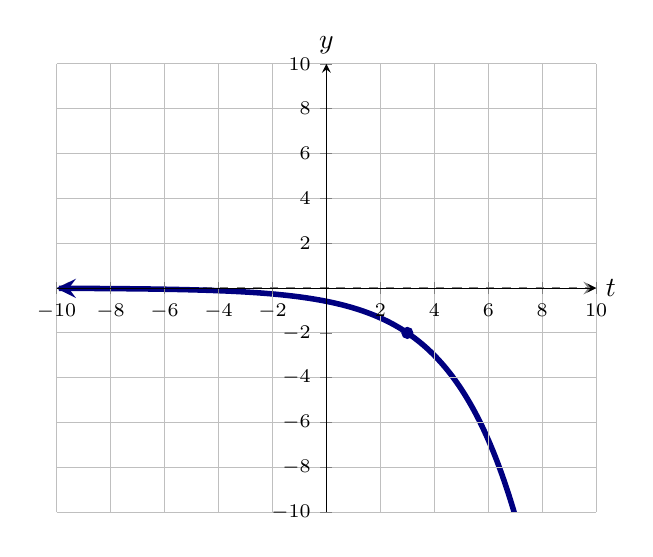
\begin{tikzpicture}
  \begin{axis}[
            domain=-10:10, ymax=10, xmax=10, ymin=-10, xmin=-10,
            axis lines =center, xlabel=$t$, ylabel=$y$, grid = major,
            ytick={-10,-8,-6,-4,-2,2,4,6,8,10},
            xtick={-10,-8,-6,-4,-2,2,4,6,8,10},
            ticklabel style={font=\scriptsize},
            every axis y label/.style={at=(current axis.above origin),anchor=south},
            every axis x label/.style={at=(current axis.right of origin),anchor=west},
            axis on top
          ]
          
          \addplot [line width=1, gray, dashed,samples=200,domain=(-10:10),<->] {0};

           \addplot [line width=2, penColor, smooth,samples=200,domain=(-10:7.5),<->] {-2 * (0.666^(3-x))};

           \addplot[color=penColor,fill=penColor,only marks,mark=*] coordinates{(3,-2)};

          


  \end{axis}
\end{tikzpicture}
\end{image}



With these ideas, we can write an algebraic analysis. \\


\end{idea}




\textbf{Domain}


$B$ is an exponential function, so its domain is $(-\infty, \infty)$.





\textbf{Zeros}


$B$ is an exponential function, so it has no zeros.




\textbf{Contiuity}


$B$ is an exponential function, so it is continuous.




\textbf{Behavior}

$B(t) = -2 \, \left( \frac{2}{3} \right)^{3-t}$ is an exponential function.  It  is either always increasing or always decreasing.


The leading coeffcient is $-2$, which is negative.  Therefore, $B$ is negative.

The leading coefficient of the linear exponent is $-1$, which is negative.  That with a base of $\frac{2}{3} < 1$ tell us us that $B$ becomes unbounded towards the positive side of the real numbers.


$B$ is a negative function that becomes unbounded toward the positive end of the real numbers.  That means $G$ is an decreasing function.



\begin{criterion}

$B$ is an exponential function, which might be compared to the basic basic exponential function $e^x$, which is a positive increasing function.\\


First, the base has been changed from $e > 1$ to $\frac{2}{3} < 1$.  That switches the behavior to decreasing.

Second, the leading coefficient of the linear exponent is $-1$, which is negative.  That switches the behavior again, back to increasing.


Third, the leading coefficient is $-2 < 0$. That switches the behavior again, back to decreasing.



\end{criterion}




\textbf{End-Behavior}


$B$ is a negative decreasing function.



\[
\lim\limits_{t \to -\infty}B(t) = \answer{0}  
\]

\[
\lim\limits_{t \to \infty}B(t) = \answer{\infty}
\]





\textbf{Local Maximum and Minimum}

Exponential functions do not have local maximums or minimums.






\textbf{Global Maximum and Minimum}

Exponential functions do not have global maximums or minimums.




\textbf{Range}



$B$ is a negative exponential function.   Its range is $(-\infty, 0)$.







\end{example}

























In the example above, we could have algebraically moved the horizontal shift to the leading coefficient.



\[
-2 \, \left( \frac{2}{3} \right)^{3-t}
\]


\[
-2 \, \left( \frac{2}{3} \right)^{3} \cdot \left( \frac{2}{3} \right)^{-t}
\]


\[
-2 \, \left( \frac{8}{27} \right)  \cdot \left( \frac{2}{3} \right)^{-t}
\]


\[
\left( \frac{-16}{27} \right)  \cdot \left( \frac{2}{3} \right)^{-t}
\]


We could have further transfered the negative sign in the exponent to the base by reciprocating the base.

\[
\left( \frac{-16}{27} \right)  \cdot \left( \frac{3}{2} \right)^t
\]



Algebra provides many tools for modifying the representing formula and altering how we think about the behavior. \\


It just depends on how you like to think of it. \\





\begin{example}  



Analyze   $K(f) = 3^{5-f}$ \\

\begin{question}
 

The base is \wordChoice{\choice{less than}\choice[correct]{greater than}} $1$.
\end{question}
\begin{question}



\begin{question}

The linear exponent is \answer{$5-f$}

\end{question}


The exponent gets big and positive when $f$ gets big and \wordChoice{\choice{positive}\choice[correct]{negative}}.
\end{question}
\begin{question}


The graph will become unbounded to the \wordChoice{\choice{right}\choice[correct]{left}}.\\
\end{question}

\begin{question}


The horizontal asymptote is $y = \answer{0}$.
\end{question}

\begin{question}


The graph will approach the asymptote to the \wordChoice{\choice[correct]{right}\choice{left}}.\\
\end{question}
\begin{question}


Our one strategic anchor point moves to $\left(\answer{5}, \answer{1}\right)$.
\end{question}
\begin{question}


The graph will become unbounded \wordChoice{\choice[correct]{up}\choice{down}}.\\
\end{question}




Graph of $y = K(f)$.

\begin{image}
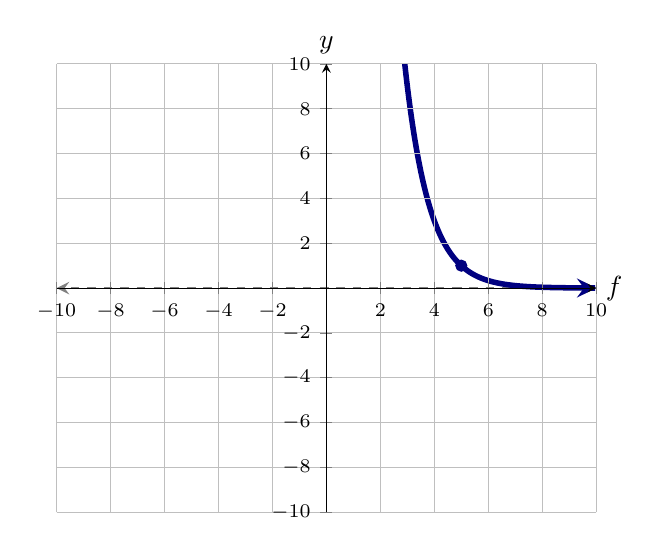
\begin{tikzpicture}
  \begin{axis}[
            domain=-10:10, ymax=10, xmax=10, ymin=-10, xmin=-10,
            axis lines =center, xlabel=$f$, ylabel=$y$, grid = major,
            ytick={-10,-8,-6,-4,-2,2,4,6,8,10},
            xtick={-10,-8,-6,-4,-2,2,4,6,8,10},
            ticklabel style={font=\scriptsize},
            every axis y label/.style={at=(current axis.above origin),anchor=south},
            every axis x label/.style={at=(current axis.right of origin),anchor=west},
            axis on top
          ]
          
          \addplot [line width=1, gray, dashed,samples=200,domain=(-10:10),<->] {0};

           \addplot [line width=2, penColor, smooth,samples=200,domain=(2.75:10),<->] {3^(5-x)};

           \addplot[color=penColor,fill=penColor,only marks,mark=*] coordinates{(5,1)};

 

  \end{axis}
\end{tikzpicture}
\end{image}





\end{example}





















\begin{center}
\textbf{\textcolor{green!50!black}{ooooo-=-=-=-ooOoo-=-=-=-ooooo}} \\

more examples can be found by following this link\\ \link[More Examples of Exponential Functions]{https://ximera.osu.edu/csccmathematics/precalculus2/precalculus2/expFunctions/examples/exampleList}

\end{center}









\end{document}
